%\section{Construction of Discrete-Time  Queueing Processes}
\section{Construction of Discrete-Time Queueing
  Processes}
\label{sec:constr-discr-time}

In this section we discuss a case as this provides real-life
motivation to analyze queueing systems. After decribing the case, we
we develop a set of recursions by which we can construct queueing
systems in discrete time.  As it turns out, this case is too hard to
analyze by mathematical means, so that simulation is the best way
forward. Interestingly, the structure of the simulation is very
simple. As such, simulation is an exceedingly convincing tool to
communicate the results of an analysis of a queueing system to
managers (and the like). 

At a mental health department five psychiatrists do intakes of future
patients to determine the best treatment process for the patients.
There are complaints about the time patients have to wait for their
first intake; the desired waiting time is around two weeks, but the
realized waiting time is sometimes more than three months. The
organization considers this is to be unacceptably long, but\ldots what to do about it?

To reduce the waiting times the five psychiatrists have various
suggestions. 
\begin{enumerate}
\item Not all psychiatrists have the same amount of time available per
  week to do intakes. This is not a problem during weeks that all are
  present. However, psychiatrists tend to take holidays, visit
  conferences, and so on. So, if the psychiatrist with the most
  intakes per week would go on leave, this might affect the behavior
  of the queue length considerably. This raises the question about the difference
  in allocation of capacity allotted to the psychiatrists. What are
  the consequences on the distribution and average of the waiting
  times if they would all have the same weekly capacity?
\item The psychiatrists tend to plan their holidays after each
  other, to reduce the variation in the service capacity. What if they
  would synchronize their holidays, to the extent possible, rather
  than spread their holidays? 
\item Finally, suppose the psychiatrists would do 2 more intakes per
  week in busy times and 2 less in quiet weeks. Assuming that the
  system is stable, i.e., the service capacity exceeds the demand,
  then on average the psychiatrists would not do more intakes, i.e.,
  their workload would not increase, but the queue length may be
  controlled better.
\end{enumerate}


To evaluate the effect of these suggestions on reducing the queueing
dynamics we develop a simple simulator and a number of plots. The
simulation of a queueing system involves the specification of its
behavior over time.  The easiest method to construct queueing
processes, hence to develop simulations, is to `chop up' time in
periods and develop recursions for the behavior of the queue from
period to period. Note that the length of such a period depends on the
case for which the model is developed.  For instance, to study
queueing processes at a supermarket, a period can consist of $5$
minutes, while for a production environment, e.g., a job shop, it can
be a day, or even a week.

Using fixed sized periods has it advantages as it does not require to
specify specific inter-arrival times or service times of individual
customers. Only the number of arrivals in a period and the number of
potential services need to be specified, which is useful since in many
practical settings, e.g., production environments, it is easier to
provide data in these terms then in terms of inter-arrival and service
times. It is, however, necessary to make some careful choices about
timing.

Let us \recall{define}
\begin{equation}
  \label{eq:30}
  \begin{split}
    a_k &= \text{number of jobs that arrive at period $k$},\\
    c_k &= \text{number of jobs that can be served during period $k$},\\
    d_k &= \text{number of jobs that depart the queue  \textit{during} period $k$},\\
    Q_k &= \text{number of jobs in queue  at the \textit{end} of period $k$}.\\
  \end{split}
\end{equation}
In the sequel we also call $a_k$ the \recall{batch} of job arrivals in
period $k$. The definition of $a_k$ is a bit subtle: we may assume
that the arriving jobs arrive either at the start or at the end of the
period. In the first case, the jobs can be served during period $k$,
in the latter case, they \emph{cannot} be served during period~$k$.


Since $Q_{k-1}$ is the queue length at the end of period $k-1$, it
must also be the queue length at the start of period $k$. Assuming
that jobs that arrive in period $k$ cannot be served in period~$k$,
the number of customers that can depart from the queue in period $k$
is
\begin{subequations}\label{eq:31}
\begin{equation}\label{eq:d_k}
d_k = \min\{Q_{k-1}, c_k\},
\end{equation}
since only the jobs that are present at the start of the period, i.e,
$Q_{k-1}$, can be served if the capacity exceeds the queue length. Now
that we know the number of departures, the queue at the end of period
$k$ is given by
\begin{equation}
    Q_k = Q_{k-1} -d_k + a_k.
\end{equation}
\end{subequations}
As an example, suppose that $c_k= 7$ for all $k$, and $a_1=5$, $a_2=4$
and $a_3=9$; also $Q_0=8$. Then, $d_1=7$, $Q_1=8-7+5=6$, $d_2 = 6$,
$Q_2=6-6+4=4$, $d_3 = 4$, $Q_3=4-4+9=9$, and so on. 

Of course we are not going to carry out these computations by
hand. Typically we use company data about the sequence of arrivals
$\{a_k\}_{k=1,2,\ldots}$ and the capacity $\{c_k\}_{k=1,\ldots}$ and
feed this data into a computer to compute the
recursions~\eqref{eq:31}. If we do not have sufficient data we make a
probability model for these data and use the computer to generate
random numbers with, hopefully, similar characteristics as the real
data. At any rate, from this point on we assume that it is easy, by
means of computurs, to obtain numbers $a_1,\ldots, a_n$ for
$n\gg 1000$, and so on.

We now show how to adapt~\eqref{eq:30} and~\eqref{eq:31} to the case
introduced above.

As a first step we model the arrival process of patients as a Poisson
process, c.f., Section~\ref{sec:poisson-distribution}. The duration of
a period is taken to be a week. The average number of arrivals per
period, based on data of the company, was slighly less than~12 per
week; in the simulation we set it to $\lambda= 11.8$ per week. We
model the capacity in the form of a matrix such that row $i$
corresponds to the weekly capacity of psychiatrist $i$:
\begin{equation*}
C = 
  \begin{pmatrix}
    1 & 1 & 1 & \ldots\\
    1 & 1 & 1 & \ldots\\
    1 & 1 & 1 & \ldots\\
    3 & 3 & 3 & \ldots\\
    9 & 9 & 9 & \ldots\\
  \end{pmatrix}
\end{equation*}
Thus, psychiatrists 1, 2, and 3 do just one intake per week, the
fourth does 3, and the fifth does 9 intakes per week. The sum over
column $k$ is the total service capacity for week $k$ of all
psychiatrists together.

With the matrix $C$ it is simple to make other capacity schemes. A
more balanced scheme would be like this:
\begin{equation*}
C = 
  \begin{pmatrix}
    2 & 2 & 2 & \ldots\\
    2 & 2 & 2 & \ldots\\
    3 & 3 & 3 & \ldots\\
    4 & 4 & 4 & \ldots\\
    4 & 4 & 4 & \ldots\\
  \end{pmatrix},
\end{equation*}

We next include the effects of holidays on the capacity. This is
easily done by setting the capacity of a certain psychiatrist to 0 in
a certain week. Let's assume that just one psychiatrist is on leave in
a week, each psychiatrist has one week per five weeks off, and the
psychiatrists' holiday schemes rotate. To model this, we set
$C_{1,1,}=C_{2,2}=\cdots=C_{1,6}=C_{2,7} =\cdots = 0$, i.e.,
\begin{equation*}
C = 
  \begin{pmatrix}
    0 & 2 & 2 & 2 & 2 & 0 & \ldots \\
    2 & 0 & 2 & 2 & 2 & 2 & \ldots\\
    3 & 3 & 0 & 3 & 3 & 3 & \ldots\\
    4 & 4 & 4 & 0 & 4 & 4 & \ldots\\
    4 & 4 & 4 & 4 & 0 & 4 & \ldots\\
  \end{pmatrix},
\end{equation*}
Hence, the total average capacity must be $4/5 \cdot (2+2+3+4+4) = 12$
patients per week.  The other holiday scheme---all psychiatrists take
holiday in the same week--corresponds to setting entire columns to
zero, i.e., $C_{i,5}=C_{i,10}=\cdots=0$ for week $5$, $10$, and so
on. Note that all these variations in holiday schemes result in the
same average capacity.

Now that we have modeled the arrivals and the capacities, we can use
the recursions~\eqref{eq:31} to simulate the queue length process for
the four different scenarios proposed by the psychiatrists, unbalanced
versus balanced capacity, and spread out holidays versus simultaneous
holidays.  The results are shown in Figure~\ref{fig:balanced}. It is
apparent that suggestions 1 and 2 above do not significantly affect
the behavior of the queue length process.  


<<echo=False,fig=False>>=
import numpy as np
import matplotlib.pylab as plt


import seaborn as sns
sns.set_context("paper")

np.random.seed(3)
a = np.random.poisson(11.8, 1000)

def computeQ(a, C, Q0=0): #  initial queue length is 0
    N = len(a)
    Q = np.empty(N) # make a list to store the values of  Q
    d = np.empty(N) # make a list to store the values of  d
    Q[0] = Q0
    for n in range(1,N):
        d[n] = min( Q[n-1]+ a[n], C[n])
        Q[n] = Q[n-1]+ a[n] - d[n]
    return Q

def unbalanced():
    p = np.empty([5,len(a)])
    p[0,:] = 1.*np.ones_like(a)
    p[1,:] = 1.*np.ones_like(a)
    p[2,:] = 1.*np.ones_like(a)
    p[3,:] = 3.*np.ones_like(a)
    p[4,:] = 9.*np.ones_like(a)
    return p

p = unbalanced()

# holidays.
for j in range(len(a)):
    Id = j%5
    p[Id,j] = 0

s = np.sum(p,axis = 0)

Qub= computeQ(a,s)

def balanced():
    p = np.empty([5,len(a)])
    p[0,:] = 2.*np.ones_like(a)
    p[1,:] = 2.*np.ones_like(a)
    p[2,:] = 3.*np.ones_like(a)
    p[3,:] = 4.*np.ones_like(a)
    p[4,:] = 4.*np.ones_like(a)
    return p

p = balanced()

for j in range(len(a)):
    Id = j%5
    p[Id,j] = 0

s = np.sum(p,axis = 0)
Qbb= computeQ(a,s)

p = unbalanced()
for j in range(int(len(a)/5)):
     p[:,5*j] = 0
s = np.sum(p,axis = 0)
Quu= computeQ(a,s)

p = balanced()
for j in range(int(len(a)/5)):
     p[:,5*j] = 0
s = np.sum(p,axis = 0)
Qbu= computeQ(a,s)

plt.figure(figsize=(6, 2))
plt.plot(Qbb, label="bal cap, spread out")
plt.plot(Qub, label="unbal capacity, simul")
plt.plot(Qbu, label="bal cap, spread out")
plt.plot(Quu, label="unbal capacity, simul")
plt.legend(loc="upper left")# , bbox_to_anchor=(1,1))
filename = "figures/balanced.pdf"
plt.savefig(filename)
plt.close()
@ 

\begin{figure}[ht]
  \centering
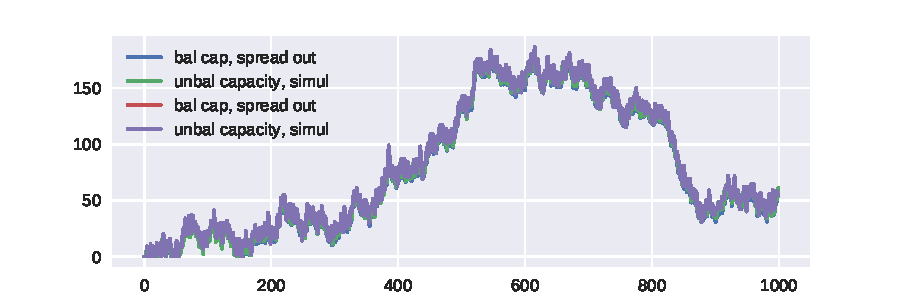
\includegraphics{balanced} 
  \caption{Effect of capacity and holiday plans}
\label{fig:balanced}
\end{figure}


Now we consider suggestion 3, which comes down to doing more intakes
when it is busy, and do less when it is quiet. A simple rule to
implement this is by considering last week's queue $Q_{n-1}$: if
$Q_{n-1}<12$, i.e., the service capacity of one week, then do $e$
intakes less. Here, $e=1$ or $2$, or perhaps a larger number; it
corresponds to the amount of control we want to exercise. When
$Q_{n-1}>24$, i.e., larger than two weeks of intakes, do $e$ intakes
more. Let's consider three different control levels, $e=1$, $e=2$, and
$e=5$; thus in the last case all psychiatrists do one extra intake.
The previous simulation shows that it is safe to disregard the holiday
plans, so just assume a flat service capacity of 12 intakes a week.

Figure~\ref{fig:intakes} shows a striking difference indeed. The queue
does not explode any more, and already taking $e=1$ has a large
influence. 

<<echo=False, fig=False>>=
def computeQExtra(a, s, e, Q0=0): #  initial queue length is 0
    N = len(a)
    Q = [0]*N # make a list to store the values of  Q
    Q[0] = Q0
    for n in range(1,N):
        q = Q[n-1]
        if  q <12:
            s[n] = max(s[n]-e,0) # protect from becoming negative
        elif q >= 24:
            s[n] += e
        Q[n] = max( q +a[n] - s[n], 0)
    return Q

np.random.seed(3)
a = np.random.poisson(11.8, 1000)
s = 12.*np.ones_like(a)
Q= computeQ(a,s)
Qe1= computeQExtra(a,s,1)
Qe2= computeQExtra(a,s,2)
Qe5= computeQExtra(a,s,5)

plt.figure(figsize=(6, 2))
plt.ylim(0, 200)
plt.plot(Q, label="Q")
plt.plot(Qe1, label="Qe1")
plt.plot(Qe2, label="Qe2")
plt.plot(Qe5, label="Qe5")
plt.legend()
filename = "figures/intakes.pdf"
plt.savefig(filename)
plt.close()
@ 

\begin{figure}[ht]
  \centering
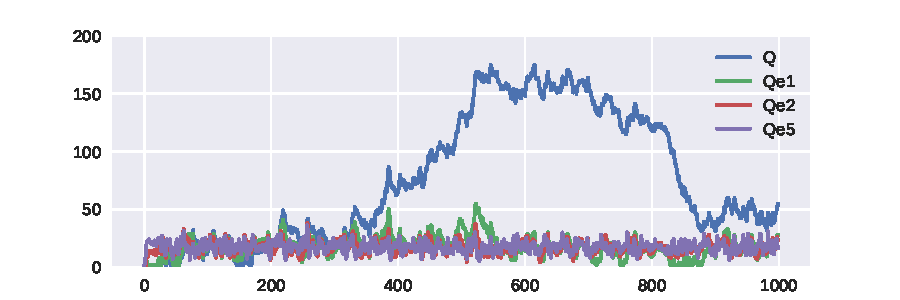
\includegraphics{intakes}  
  \caption{Controling the number of intakes}
\label{fig:intakes}
\end{figure}

From the simulation experiment we learn that changing holiday plans or
spreading the work over multiple servers, i.e., psychiatrists, does
not significantly affect the queueing behavior.  However, controlling
the service rate as a function of the queue length improves the
situation quite dramatically. 

Thus, we made models for the arrival and service processes and then
developed a simple recursion of the type~\eqref{eq:31} to
\recall{construct} a queueing process. Finally, for the analysis, we
made plots of these processes. 


In more abstract terms the study of queueing system is focussed on
studying the probabilistic properties of the queueing length process
and related concepts such as waiting time, server occupancy, fraction
of customers lost, and so on. Once we have constructed the queueing
process we can compute all performance measures of relevance, such as
the average waiting time,
c.f. Section~\ref{sec:limits-of-emperical}. If it turns out that the
performance of the system is not according to what we desire, we can
change parts of the system with the aim to improve the situation and
assess the effect of this change.  For instance, if the average
waiting time is too long, we might add service capacity with the aim
to reduce the service times, hence reduce the average waiting
time. With simulation it is easy to study the effect of, hence
evaluate, such decisions.

Observe that, even with these simple recursions, we can obtain
considerable insight into this, otherwise, very complicated controlled
queueing process. (If the reader doubts the value of simulation, s/he
should try to develop other mathematical methods to analyze
multi-server queueing system with vacations, of which this is an
example. Warning, do not even attempt: you'll fail as it is most
probably too hard.) The simplicity of the recursions is deceitful, but
with these simple recursions we can analyse many practical queueing
situations. Together with students the author applied it numerous
times, for instance,
\begin{itemize}
\item Should a certain hospital invest in a new MRI scanner to reduce
  waiting times?
\item When to switch on and off a tin bath at an eletronics component factory?
\item What is the effect of reducing the number of jobs in a paint
  factory?
\item Post parcel routing in a post sorting center.
\item Controlling inventories at various companies.
\item Throughput time analysis at courts.
\end{itemize}
And so on, and so on. The recursions are indeed astoningly useful. We
therefore urge the reader to practice with this type of queueing
modeling. The exercises below provide ample material for this purpose.

In passing we remark that yet more powerful simulations can be carried
out with, so-called, event-based simulations. We refer to
\cite[Section 4.5]{hall91:_queuein_method_servic_manuf} for a general
description of this technique. The author applied this to quite complicated queueing networks:
\begin{itemize}
\item Analysis of the packaging process of a large beer factory.
\item Performance analysis of large telecommunication networks
\item Optimization of truck routing and queueing for a sugar factory.
\end{itemize}
Due to lack of time, we decided not to include this. 

The reader should understand from the above case that, once we have
the recursions, we can analyze the system and make plots to evaluate
suggestions for improvement.  Thus, getting the recursions is crucial
to construct, i.e., model, queueing processes. For this reason, most
of the exercises below focus on obtaining recursions for many
different queueing systems.

\begin{question}
 What are the consequences of setting
    $d_k = \min\{Q_{k-1}+a_k,  c_k\}$ rather than the definition~\eqref{eq:d_k}?
\begin{solution}
 The assumption is that the jobs arrive at the start of period
    $k$, before service in period $k$ starts, rather than at the end
    of the period. Therefore the arrivals at period $k$ can also be
    served during period $k$.
\end{solution}
\end{question}


\begin{question} (Queue with Blocking) Consider a queueing system
  under daily review, i.e., at the end of the day the queue length is
  measured. We assume that at the end of the day no jobs are still in
  service. We assume that jobs that arrive at day $n$ cannot be served
  in day $n$. The queue length cannot exceed level $K$.  Formulate a
  set of recursions to cover this case.
  \begin{solution}

    All jobs that arrive such that the queue become larger than $K$
    must be dropped. Thus, the accepted arrivals $a_n'$ in week $n$
    are such that $a_n' = \min\{a_n, K-Q_{n-1}\}$, where $a_n$ are all
    arrivals in period $n$.  The rest of the recursions remain the
    same.

  \end{solution}
\end{question}


\begin{question}
  (Yield loss) A machine produces items, but part of the items turn
  out to be faulty, and have to be made anew. Make assumptions about
  the failure process, and develop a set of recursions to cover this
  case.
  \begin{solution}
    Let's assume that a fraction $p$ of the jobs is lost each
    period. We can make $p$ time-dependent if we like, but for the
    moment we don't. The amount produced in period $k$ is $d_k$. Thus,
    $p d_k$ is the amount lost, neglecting rounding errors for the
    moment. Thus, $p d_k$ items have to be fed back to the system in
    the next period to be remade. Therefore the total amount of
    arrivals in period $k+1$ is $a_{k+1}'=a_{k+1}+pd_k$, i.e., the
    external arrivals plus the extra items. Now use the standard
    recursions but with the $\{a_{k}'\}$ rather than $\{a_k\}$. 

    Can you use these recursions to show that the long-run average
    service capacity $n^{-1}\sum_{i=1}^n c_i$ must be larger than
    $\lambda(1+p)$.
      \end{solution}
\end{question}

\begin{question}
  (Rework) A machine produces items, but part of the items do not meet
  the quality requirements after the first service but need some extra
  service time but less than an entirely new arriving job. Make a
  model to analyze this case. Compare this case with the yield loss
  problem above. 

  Let's assume that the repair of a faulty requires half of the work
  of a new job, and that the faulty jobs are processed with priority
  over the new jobs. (There are of course many different policies to
  treat rework; here we make this assumption. For your interest:
  another possibility is that faulty items are processed at the end of
  the day. Yet another possibility is that faulty items are collected
  until there are $N$, say, and then the entire batch of $N$ is
  repaired.)

  \begin{solution}
    Suppose again that a fraction $p$ is faulty. Since these faulty
    items require less processing time than a new job, the service
    capacity $c_k$, i.e., the number of jobs that can be processed in
    period $k$, is a bit bigger; part of the capacity is spent at new
    jobs but another part is spent on the faulty jobs. Let's assume
    that the repair of a faulty requires half of the work of a new
    job, and that the faulty jobs are processed with priority over the
    new jobs. Assume queue $A$ contains the faulty items, and queue
    $B$ the new jobs. Then the recursions become:
\begin{equation*}
  \begin{split}
    d_{k,A} &= \min\{Q_{k-1, A}, 2c_k\}, \text{ as faulty jobs require half of the processing time})\\
    c_{k,B} &= c_k - d_{k,A}/2, \\
    d_{k,B} &= \min\{Q_{k-1, B}, c_{k,B}\}, \\
    Q_{k,A} &= Q_{k-1, A} + a_{k,A} - d_{k,A}, \\
    Q_{k,B} &= Q_{k-1, B} + a_{k,B} - d_{k,B}.
  \end{split}
\end{equation*}

  \end{solution}
\end{question}


\begin{question}(Cost models) A single-server queueing station
  processes customers. At the start of a period the server capacity is
  chosen, so that for period $k$ the capacity is $c_k$. Demand that
  arrives in a period can be served in that period. It costs $\beta$
  per unit time per unit processing capacity to operate the machine,
  i.e., to have it switched on. There is also a cost $h$ per unit time
  per job in the system. Make a cost model to analyze the long-run
  average cost for this case.
  \begin{solution}
First consider the dynamics of the queue. Since the capacity is chosen at the start of the period:
\begin{align*}
  d_k &= \min\{Q_{k-1}+a_k, c_k\} \\
Q_k &= Q_{k-1}+a_k - d_k.
\end{align*}
The cost to operate the server during period $k$ is $\beta c_k$.
Thus, the total cost up to some time $T$ for the server must be
$\beta \sum_{k=1}^T c_k$. In period $k$ we also have to pay $h Q_k$,
since $h$ is the cost per customer per period in the system. Thus, the
long-run average cost is
    \begin{equation*}
      \frac 1T\sum_{k=1}^T \left(\beta c_k + h Q_k\right).
    \end{equation*}

    It is an interesting problem to find a policy that minizes (the
    expectation of) this cost. The policy is such that the capacity
    for period $k$ can be chosen based on the queue length $Q_{k-1}$
    and \emph{estimates} of the demands
    $\hat d_k, \hat d_{k+1}, \ldots$. This problem is not easy, as far as I can see. 

  \end{solution}
\end{question}

\begin{question}(N-policies) A machine can switch on and off. If the
  queue length hits $N$, the machine switches on, and if the system
  becomes empty, the machine switches off. It costs $K$ to switch on
  the machine. There is also a cost $\beta$ per unit time while the
  machine is switched on, and it costs $h$ per unit time per customer
  in the system. Make a cost model. 
  \begin{solution}
    First we need to implement the N-policy. For this we need an extra
    variable to keep track of the state of the server. Let $I_k=1$ if the machine is on in period $k$ and $I_k=0$ if it is off. Then $\{I_k\}$ must satisfy the relation
    \begin{equation*}
      I_{k+1} =
      \begin{cases}
        1 & \text{ if } Q_{k} \geq N,\\
        I_k & \text{ if } 0< Q_{k} <N,\\
        0 & \text{ if }  Q_{k} =0,\\
      \end{cases}
    \end{equation*}
and assume that $I_0 =0$ at the start, i.e., the machine if off. Thus, we can write:
\begin{equation*}
  I_{k+1} = \1{Q_k\geq N} + I_k \1{0<Q_k<N} + 0\cdot \1{Q_k = 0}.
\end{equation*}
With $I_k$ it follows that $d_k =\min\{Q_{k-1}, I_k c_k\}$, from which
$Q_k$ follows, and so on.

The machine cost for period $k$ is $\beta I_k$, because only when the
machine is on we have to pay $\beta$, and the queueing cost is
$h Q_k$. To determine the total switching cost is harder as we need to
determine how often the machine has been switched on up to time
$T$. Observe that the machine is switched on in period $k$ if
$I_{k-1} = 0$ and $I_k=1$. Thus, whenever $I_k - I_{k-1}=1$ the
machine is switched on, when $I_k - I_{k-1}=0$ the state of the
machine remains the same, and if $I_k - I_{k-1} = -1$ the machine is
switched off. In other words $\max\{I_k - I_{k-1},0\}$ captures what
we need. The total cost up to time $T$ becomes:
\begin{equation*}
  \sum_{k=1}^T \left(\beta I_k + h Q_k + K\max\{I_k - I_{k-1}, 0\}\right).
\end{equation*}
  \end{solution}
\end{question}


\begin{question}(Queue with setups)[use=false]
  One server serves two parallel queues, one at a time. After serving
  a batch of 20 jobs of one queue the server moves to the other
  queue. The change of queue requires one period setup time.
  \begin{solution}
    \tbd.
  \end{solution}
\end{question}


\begin{question}
  How would you model (in terms of recursions) a server whose capacity depends on the queue length? 
  \begin{solution}
    One model could be to let the server only switch on when the queue
    is larger than some threshold $t$, and when the server is on, it
    works at rate $c$ per period. In that case,
    $c_k = c\1{Q_{k-1} > t}$.
  \end{solution}
\end{question}

\begin{question}(Fair queueing) One server serves two queues. Each
  queue receives service capacity in proportion to its queue length. Derive a set of recursions to analyze this situation.
  \begin{solution}
    Let $c_k^i$ be the capacity allocated to queue $i$ in period $k$. The fair rule gives that 
    \begin{equation*}
      c_k^1 = \frac{Q_{k-1}^1}{Q_{k-1}^1 + Q_{k-1}^2} c = c - c_k^2. 
    \end{equation*}
Then, 
\begin{equation*}
  \begin{split}
      d_k^1 &= \min\{Q_{k-1}^1, c^1_k\}, \\
Q_k^1 &= Q_{k-1}^1+a_k^1  - d_k^1,
  \end{split}
\end{equation*}
and likewise for the other queue.
  \end{solution}
  \end{question}

  \begin{question} (Priority queuing) Another interesting situation is
    a system with two queues served by one server, but such that one
    queue gets non-preemptive priority over the other queue. Again
    find a set of recursions to describe this case.
    \begin{solution}
 If other choices for the division of the production capacity
  over the types is made (for instance strict priority to type A), it
  is necessary to split the queue in front of the mixing station into
  two separate queues $Q_A$ and $Q_B$, one for each type.  The rules
  below implement a strict priority rule for jobs type A.
\begin{equation*}
  \begin{split}
    d_{k,A} &= \min\{Q_{k-1, A}, c_k\}, \\
    c_{k,B} &= c_k - d_{k,A}, \\
    d_{k,B} &= \min\{Q_{k-1, B}, c_{k,B}\}, \\
    Q_{k,A} &= Q_{k-1, A} + a_{k,A} - d_{k,A}, \\
    Q_{k,B} &= Q_{k-1, B} + a_{k,B} - d_{k,B}.
  \end{split}
\end{equation*}
As an aside, another interesting rule to distribute the capacity $c_k$
over the queues could be based on the principle of \textit{ equal
  division of the contested sum}. This principle is based on game
theoretic ideas. Aumann and Maschler applied this principle to clarify
certain division rules discussed in the Talmud to divide the legacy
among a number of inheritors, each having a different claim size.
    \end{solution}
\end{question}



\begin{question} 
  (Queues with reserved service capacity) Consider a single-server that
  serves two parallel queues. Each queue receives a minimal service
  capacity every period. Reserved capacity unused for one queue can be
  used to serve the other queue. Any extra capacity beyond the
  reserved capacity is given to queue A with priority. Formulate a set
  of recursions to analyze this situation.
  \begin{solution}
    First determine how much capacity queue $B$ minimally needs in
    period $k$:
    \begin{equation*}
      c_{k,B} = \min\{Q_{ k-1, B}, r_B\}
    \end{equation*}
    Observe that, since $c_k \geq r_A + r_B$, this rule ensures that
    queue A receives at least its reserved capacity $r_A$. 

    Since queue A is served with priority, we first give all capacity,
    except what queue B minimally needs, to queue A:
    \begin{equation*}
d_{k,A} = \min\{Q_{k-1, A}, c_k-c_{k,B}\}.
\end{equation*}
And then we can give any left over capacity to queue B, if needed. 
\begin{align*}
d_{k,B} &= \min\{Q_{k-1, B}, c_k-d_{k,A}\}.
\end{align*}

    An example is the weekly capacity offered by a psychiatrist at a
    hospital. Part of the weekly capacity is
    reserved/allocated/assigned to serve certain patients groups. For
    instance, each week the psychiatrist does at most five intakes of
    new patients, provided there are any, and the rest of the capacity
    is used to treat other patients. The existing patients can also be
    divided in different groups, each receiving a minimal capacity. It
    there less patients of some group, then the capacity can be
    planned/given to other patient groups. 

  \end{solution}
\end{question}


\begin{question} 
  (Queue with protected service capacity, lost capacity) Consider a
  single-server that serves two parallel queues. Each queue receives a
  minimal service capacity every period. Reserved capacity unused for
  one queue cannot be used to serve the other queue. Any extra
  capacity beyond the reserved capacity is given to queue A with
  priority. Formulate a set of recursions to analyze this situation.
  \begin{solution}
    Let $r_A$ be the reserved for queue A, and likewise for $r_B$. We
    assume of course that $c_k\geq r_A + r_B$, for all $k$. 

Queue A can use all capacity, except what is reserved for queue B: 
\begin{equation*}
  d_{k,A} = \min\{Q_{A, k-1}, c_k - r_B\}.
\end{equation*}
Observe that, since $c_k \geq r_A + r_B$, this rule ensures that queue
A receives at least its reserved capacity $r_A$.

Queue $B$ cannot receive more than $c_k-r_A$, since $r_A$ is allocated
to queue A, and if queue $A$ does not use all of $r_A$, then the
surplus is lost. Also, queue $B$ cannot get more than $c_k - d_{k,A}$
as this is what remains after serving queue $A$. Thus, letting
$c_{k,B} = \min\{c_k-r_A, c_k-d_{k,A}\} = c_k - \max\{r_A, d_{k,A}\}$,
we see that for queue B:
\begin{equation*}
  d_{k,B} = \min\{Q_{B, k-1}, c_{k,B}\}.
\end{equation*}

An example can be the operation room of a hospital. There is a weekly
capacity, part of the capacity is reserved for emergencies. It might
not be possible to assign this reserved capacity to other patient
groups, because it should be available at all times for emergency
patients. A result of this is that unused capacity is lost.  

In practice it may not be as extreme as in the model, but still part
of the unused capacity is lost. `Use it, or lose it', is what often,
but not always, applies to service capacity.
  \end{solution}
\end{question}




\begin{question}(Tandem  networks) 
  Consider a production network with two production stations in
  tandem, that is, the jobs processed by station A are in the next
  period to the downstream Station B.  Extend the recursions of
  \eqref{eq:31} to simulate this situation.
\begin{solution}
  Let $a_k$ be the external arrivals at station A. Then:
\begin{equation}
  \begin{split}
    d^A_k &= \min\{Q_{k-1}^A, c_k^A\}, \\
    Q_k^A &= Q_{k-1}^A -d_k^A + a_k.
  \end{split}
\end{equation}
The departures of the first station during period $k$ are the arrivals
at station $B$ at the end of period $k$, i.e., $a_k^B =
d_{k}^A$. Thus,
\begin{equation}
  \begin{split}
    a_k^B &= d_{k}^A,\\
    d^B_k &= \min\{Q_{k-1}^B, c_k^B\}, \\
    Q_k^B &= Q_{k-1}^B -d_k^B + a_k^B.
  \end{split}
\end{equation}
\end{solution}
\end{question}

\begin{question} (A tandem queue with blocking)
  Consider a production network with two production stations in tandem
  with blocking: when intermediate queue, i.e., the queue front of
  Station B, exceeds some level $M$, then station A has to stop
  producing, and when $Q^B_k < M$ station A is not allowed to produce
  more then the intermediate queue can contain. Extend the recursions
  of \eqref{eq:31} to simulate this situation.
\begin{solution}
\begin{equation}
  \begin{split}
    d^A_k &= \min\{Q_{k-1}^A, c_k^A, M-Q^B_{k-1}\}, \\
    Q_k^A &= Q_{k-1}^A -d_k^A + a_k, \\
    a_k^B &= d_{k}^A,\\
    d^B_k &= \min\{Q_{k-1}^B, c_k^B\}, \\
    Q_k^B &= Q_{k-1}^B -d_k^B + a_k^B.
  \end{split}
\end{equation}
This is a bit subtle: since there is room $M-Q^B_{k-1}$ at the
intermediate buffer and $d_k^A \leq M-Q^B_{k-1}$, we know that in the
worst case, i.e., when $c_k^B=0$, still $Q^B_k = Q_{k_1}^B +
d_k^A$.
Thus, we are sure that the queue length of the intermediate queue will
not exceed $M$.

There is still  a small problem: What if for the first initial periods  $M<Q^B_{k-1}$. Then $M-Q^B_{k-1}<0$ and then by the specification above, $d_k^A < 0$. This is not what we want. Therefore, 
\begin{equation*}
  d^A_k = \min\{Q_{k-1}^A, c_k^A, \max\{M-Q^B_{k-1}, 0\}\}.
\end{equation*}
\end{solution}
\end{question}

\begin{question} (Merging departure streams)
  Consider another production situation with two machines, A and B
  say, that send their products to Station C. Derive a set of
  recursion relations to simulate this system. 
\begin{solution}
Realize that Stations A and B have their own arrivals. 
\begin{equation}
  \begin{split}
    d^A_k &= \min\{Q_{k-1}^A, c_k^A\}, \\
    Q_k^A &= Q_{k-1}^A -d_k^A + a_k^A, \\
    d^B_k &= \min\{Q_{k-1}^B, c_k^B\}, \\
    Q_k^B &= Q_{k-1}^B -d_k^B + a_k^B, \\
    a_k^C &= d_{k}^A+d_{k}^B,\\
    d^C_k &= \min\{Q_{k-1}^C, c_k^C\}, \\
    Q_k^C &= Q_{k-1}^C -d_k^C + a_k^C.
  \end{split}
\end{equation}
\end{solution}
\end{question}

\begin{question} (Merging incoming streams)
  Consider a single-server queue that servers two customer `streams'
  in a FIFO discipline. Thus, both streams enter one queue that is
  served by the server. Let $\{a_k^a\}$ be the number of arrivals of
  stream $a$ in period $k$ and $\{a_k^b\}$ be the number of arrivals
  of stream $b$. Find a set of recursions by which it becomes possible
  to analyze the waiting time distribution of each of the streams.
  \begin{solution}
    The behavior of the queue length  process is easy: 
    \begin{equation*}
      \begin{split}
      d_k &= \min\{Q_{k-1}, c\}, \\
Q_k &= Q_{k-1}+a_k^a + a_k^b - d_k.
      \end{split}
    \end{equation*}

    To determine the waiting times, observe that any arrival in period
    $k$, independent of the stream, has to wait until all jobs at the
    start of the period in queue, i.e., $Q_{k-1}-d_k$, are cleared;
    note that we assume here that the jobs served in period $k$ depart
    at the start of the interval. Thus, the minimal waiting time is
    $l_{k,-} = \lfloor (Q_{k-1}-d_k)/c\rfloor$.  Similarly, the
    maximal waiting time is $l_{k,+} = \lceil Q_k /c\rceil$.

    The only remaining problem is to make a model to `distribute' the
    time between $l_{k,-}$ and $l_{k,+}$ over the two streams. One way
    is to give priority to $a$ customers.  Making this completely
    explicit, so that the recursion can be fed to the computer,
    requires still a bit of work.  It is important to understand the
    trick we will discuss now because we will use it to model queueing
    systems with batching. Observe that the first job of the $a$
    stream only has to wait for $l_{k,-}$, the second job must wait $l_{k,-}+1$, and so on. Thus, the average waiting is 
    \begin{equation*}
      \frac{l_{k,-} + (l_{k,-} + 1) + \ldots + (l_{k,-} + a_k^a-1)}{a_k^a} = l_{k,-} + \frac{a_k^a-1}2.
    \end{equation*}
Similarly, the average waiting time for the $b$ jobs must be
    \begin{equation*}
      \frac{l_{k,-} + a_k^a + l_{k,-} + a_k^a + 1 + \ldots + l_{k,-} + a_k^a + a_k^b -1}{a_k^b} = l_{k,-} + a_k^a + \frac{a_k^b-1}2.
    \end{equation*}

    Another model is to assume that the waiting time is simply
    averaged over the jobs. Then each job perceives a waiting time of
    \begin{equation*}
      \frac{l_{k,-} + l_{k,+}}2.
    \end{equation*}
  \end{solution}
\end{question}



\begin{question} (Splitting streams)
  Consider a machine (a paint mixing machine) that produces products
  for two separate downstream machines A and B (two different paint
  packaging machines), each with its own queue.  Suppose we want to
  analyze the queue in front of station A. For this we need to know
  the arrivals to station A, that is, the departures of the mixing
  station that go to station A. Provide a set of recursions to
  simulate this system.
  \begin{solution}
\begin{enumerate}
\item Realize that the recursions of Eq~\eqref{eq:31} applied to the
  queueing situation at the first machine provide us with the total
  number of departures $d_k$ during period $k$. However, it does not
  tell us about the type of these departures. Thus, to compute the
  queue in front of station A, we need do know the number of
  departures of type A, rather than the total number of departures of
  the first station.
\item It is reasonable that the number of jobs of type $A$ in queue at
  the first station is equal to
  \begin{equation*}
  Q_k \frac{\lambda_A}{\lambda_A + \lambda_B}.
  \end{equation*}
  It is therefore reasonable to assume that the capacity $c_k$ of the
  first station is also shared in this proportion to type A and B
  jobs. Thus, the number of departures to station $A$ is
  \begin{equation*}
    d_k(A) = \frac{\lambda_A}{\lambda_A+\lambda_B} \min\left\{ Q_{k-1}, c_k\right\}.
  \end{equation*}
 The rest of the recursions is very similar to what we did in earlier exercises.
\end{enumerate}
  \end{solution}
\end{question}



\begin{question}(Inventory control) The recursions used in the
  exercises above can also be applied to analyze inventory control
  policies. Consider a production system that can produce maximally
  $M_k$ items per week during normal working hours, and maximally
  $N_k$ items during extra (weekend and evening hours). Let, for
  period $k$,
  \begin{align*}
    D_k &= \text{Demand in  week $k$}, \\
    S_k &= \text{Sales, i.e., number of items sold, in week $k$}, \\
    r_k &= \text{Revenue per item sold in week $k$}, \\
    X_k &= \text{Number of items produced in week $k$  during normal hours}, \\
    Y_k &= \text{Number of items produced in week $k$ during extra  hours}, \\
    c_k &= \text{Production cost per item during normal  hours}, \\
    d_k &= \text{Production cost per item during extra  hours}, \\
    h_k &= \text{holding cost per  item, due at the end of week $k$}, \\
    I_k &= \text{On hand inventory level at the end of week $k$}. \\
  \end{align*}
  Management needs a production plan that specifies for the next $T$
  weeks the number of items to be produced per week. Formulate this
  problem as an LP problem, taking into account the inventory
  dynamics.  

\hint{Formuale the decision variables/controls, the
    objective and the constraints.}

  \begin{solution}
    The decision variables are $X_k$, $Y_K$ and $S_k$ (note, it is not
    necessary to meet all demand:  the production cost and profit
    may vary per period.)  The objective is 
    \begin{equation*}
      \max \sum_{k=1}^T (r_kS_k -c_k X_k - d_k Y_k - h_k I_k).
    \end{equation*}
The constraints are 
\begin{align*}
  0&\leq S_k \leq D_k, \\
  0&\leq X_k \leq M_k, \\
  0&\leq Y_k \leq N_k, \\
  I_k&=I_{k-1}+X_k+Y_k - S_k. \\
I_k &>= 0.
\end{align*}
  \end{solution}
\end{question}

\begin{question} (Estimating the lead time distribution.)  Take
  $d_k = \min\{Q_{k-1}+a_k, c_k\}$, and assume that jobs are served in
  FIFO sequence. Find an expression for the shortest possible waiting
  time $W_-(k)$ of a job that arrives at time $k$, and an expression
  for the largest possible waiting time $W_+(k)$
  \hint{Consider a numerical example. Suppose $Q_{k-1}=20$. Suppose
    that the capacity is $c_k=3$ for all $k$. Then a job that arrives
    in the $k$th period, must wait at least $20/3$ (plus rounding)
    periods before it can leave the system. Now generalize this
    numerical example.}
    \begin{solution}
    A job that arrives at time $k$ cannot be served before period
    \begin{equation*}
    W_-(k):= \max\left\{l: \sum_{i=k}^{k+l} d_i < Q_{k-1}\right\},
    \end{equation*}
and it must have been  served before period
    \begin{equation*}
      W_+(k):= \min\left\{l: \sum_{i=k}^{k+l} c_i \geq
        Q_{k}\right\}.
    \end{equation*}
    Thus, the waiting time of jobs arriving in period $k$ must lie in
    $[W_-(k), W_+(k)]$.
  \end{solution}
\end{question}

\begin{question}
  Implement Eqs.~\ref{eq:31} in a computer program and simulate a
  simple single-server queueing system. 
  \begin{solution}
    Here is an example in python; please read the code to see how I
    approach the problem. The code is really easy, as it is nearly
    identical to the mathematical specification. You don't have to
    memorize the specific syntax of the code, of course, but it is (at
    least I find it) interesting to see how little code is actually
    necessary to set things up.


    Below I fix the seed of the random number generator to ensure that
    I always get the same results from the simulator.  The arrival
    process is Poisson, and the number of services is fixed to 21 per
    period. I use \texttt{Q = np.zeros\_like(a)} to make an array of the
    same size as the number of arrival $a$ initially set to zeros. The
    rest of the code is nearly identical to the formulas in the text.

<<>>=
import numpy as np

np.random.seed(3) # fix the seed

labda = 20
mu = 21
@

These are the number of arrivals in each period.

<<term=True>>=
a = np.random.poisson(labda, 10)
a
@

The number of potential services
<<term=True>>=
c = mu * np.ones_like(a)
c
@ 

Now for the queueing recursions:

<<>>=
Q = np.zeros_like(a)
d = np.zeros_like(a)
Q[0] = 10  # initial queue length

for k in range(1, len(a)):
    d[k] = min(Q[k - 1], c[k])
    Q[k] = Q[k - 1] - d[k] + a[k]
@

These are the departures for each period:
<<term=True>>=
d
@

The queue lengths
<<term=True>>=
Q
@

<<term=True>>=
loss = (Q > 20)
loss
loss.sum()
@

Here I
define loss as the number of periods in which the queue length exceeds
20. Of course, any other threshold can by taken. Counting the number
of such periods is very easy in python: \texttt{(Q>20)} gives all
entries of $Q$ such $Q>20$, the function \texttt{sum()} just adds
them. 


Now all statistics:

<<term=True>>=
d.mean()
Q.mean()
Q.std()
(Q > 20).sum()
@

Since this is a small example, the mean number of departures, i.e.,
\texttt{d.mean()}, is not equal to the arrival rate $\lambda$.  
Likewise for the computation of the mean, variance, and other
statistical functions. 

Now I am going to run the same code, but for a larger instance. 

<<>>=
num = 1000
a = np.random.poisson(labda, num)
c = mu * np.ones_like(a)
Q = np.zeros_like(a)
d = np.zeros_like(a)
Q[0] = 10  # initial queue length

for k in range(1, len(a)):
    d[k] = min(Q[k - 1], c[k])
    Q[k] = Q[k - 1] - d[k] + a[k]
@

<<term=True>>=
d.mean()
Q.mean()
Q.std()
(Q > 30).sum()/num * 100
@


I multiply with 100 to get a percentage. Clearly, many jobs see a long
queue, the mean is already some 24 jobs. For this arrival rate a
service capacity of $\mu=21$ is certainly too small. 

Next, an example with the same arrival pattern but with a Poisson
distributed number of jobs served per day, so the service rate is
still $21$, but the period capacity $c$ is random variable with
Poisson distribution with $P(21)$

<<fig = False, width = '12 cm'>>=
c = np.random.poisson(mu, num)
Q = np.zeros_like(a)
d = np.zeros_like(a)
Q[0] = 10  # initial queue length

for k in range(1, len(a)):
    d[k] = min(Q[k - 1], c[k])
    Q[k] = Q[k - 1] - d[k] + a[k]
@

<<term=True>>=
d.mean()
Q.mean()
Q.std()
(Q > 30).sum()/num * 100
@

Compared to the case with constant service capacity, i.e., $c=21$ in
each period, we see that the average waiting time increases, just as
the number of periods in which the queue length exceeds 30. Clearly,
variability in service capacity does not improve the performance of
the queueing system, quite on the contrary. In later sections we will
see why this is so.

You can try to implement some of the other cases of the exercises in
this section and analyze them in the same way. Hopefully you
understand from this discussion that once you have the recursions to
construct/simulate the queueing process, you are `in business'. The
rest is easy: make plots, do some counting, i.e., assemble statistics,
vary parameters for sensitivity analysis, and so on.

  \end{solution}
\end{question}


%%% Local Variables:
%%% mode: latex
%%% TeX-master: "book"
%%% End:
